\documentclass[12pt,a4paper]{article}
\usepackage[left=2cm,right=2cm,top=2cm,bottom=2cm]{geometry}
\usepackage[utf8]{inputenc}
\usepackage[T2A]{fontenc}
\usepackage{amsmath}
\usepackage{amssymb}
\usepackage{graphicx}
\usepackage[russian]{babel}
\usepackage{indentfirst}
\usepackage{listings}
\usepackage{xcolor}
\usepackage{hyperref}

\hypersetup{
  colorlinks=true,
  urlcolor= blue,
  citecolor=blue,
  linkcolor= blue,
}

\title{Отчет по лабораторным работам №1-2 по дисциплине "Математическая статистика"}
\author{Скворцов Владимир Сергеевич (5030102/10201)}
\date{\today}

\begin{document}

	\begin{titlepage}

		\Large

		\begin{center}
			Санкт-Петербургский \\ Политехнический университет Петра Великого

			\vspace{10em}

			\textbf{Отчет по лабораторным работам №1-2} \\
			\textbf{по дисциплине}\\
			"\textbf{Математическая статистика}"

			\vspace{2em}

		\end{center}

		\vspace{6em}

		\newbox{\lbox}
		\savebox{\lbox}{\hbox{Скворцов Владимир Сергеевич}}
		\newlength{\maxl}
		\setlength{\maxl}{\wd\lbox}
		\hfill\parbox{12cm}{
			\hspace*{3cm}\hspace*{-5cm}Студент:\hfill\hbox to\maxl{Скворцов Владимир Сергеевич\hfill}\\
			\hspace*{3cm}\hspace*{-5cm}Преподаватель:\hfill\hbox to\maxl{Баженов Александр Николаевич}\\
			\\
			\hspace*{3cm}\hspace*{-5cm}Группа:\hfill\hbox to\maxl{5030102/10201}\\
		}

		\vspace{\fill}

		\begin{center}
			Санкт-Петербург \\ 2024
		\end{center}

	\end{titlepage}

	\tableofcontents\newpage

	\section{Постановка задачи}
	\subsection{Описательная статистика}
	Для 5 распределений:\\
	\begin{itemize}
	\item Нормальное распределение $N(x, 0, 1)$
	\item распределение Коши $C(x, 0, 1)$
	\item Распределение Стьюдента $t(x, 0, 3)$ с тремя степенями свободы
	\item Распределение Пуассона $P(k, 10)$
	\item Равномерное распределение $U(x, -\sqrt3, \sqrt3)$
	\end{itemize}
	Сгенерировать выборки размером 10, 50, 1000 элементов.\\
	Построить на одном рисунке гистограмму и график плотности распределения.

	\subsection{Точечное оценивание характеристик положения и рассеяния}
	Сгенерировать выборки размером 10, 50, 1000 элементов.\\
	Для каждой выборки вычислить следующие статистические характеристики положения данных: $\overline{x}$, $med\:x$, $z_{Q}$, $z_{R}$, $z_{tr}$. Повторить такие вычисления 1000 раз для каждой выборки и найти среднее характеристик положения и их квадратов: $E(z) = \bar{z}$. Вычислить оценку дисперсии по формуле $D(z) = \overline{z^2} - \overline{z}^2$.

	\section{Теоретическое обоснование}
	\subsection{Функции распределения}
	\begin{itemize}
		\item Нормальное распределение

		\begin{equation} \label{eq:normal}
			N(x, 0, 1) = \frac{1}{\sqrt{2\pi}}e^\frac{-x^2}{2}
		\end{equation}

		\item Распределение Коши

		\begin{equation} \label{eq:cauchy}
			C(x, 0, 1) = \frac{1}{\pi}\frac{1}{x^2+1}
		\end{equation}

		\item Распределение Стьюдента $t(x, 0, 3)$ с тремя степенями свободы

		\begin{equation} \label{eq:student}
			t(x, 0, 3) = \frac{6\sqrt3}{\pi(3 + t^2)^2}
		\end{equation}

		\item Распределение Пуассона

		\begin{equation} \label{eq:poisson}
			P(k, 10) = \frac{10^k}{k!}e^{-10}
		\end{equation}

		\item Равномерное распределение

		\begin{equation} \label{eq:uniform}
			U(x, -\sqrt3, \sqrt3) = \begin{cases}
				\frac{1}{2\sqrt3} & \mbox{при} \; |x| \leq \sqrt3\\
				0 & \mbox{при} \; |x| > \sqrt3
			\end{cases}
		\end{equation}
	\end{itemize}

	\subsection{Характеристики положения и рассеяния}

	\begin{itemize}
		\item Выборочное среднее

		\begin{equation} \label{eq:mean}
			\overline{x} = \tfrac{1}{n}\sum_{i = 1}^{n}x_i
		\end{equation}

		\item Выборочная медиана

		\begin{equation} \label{eq:median}
			med\ x = \left\{
			\begin{array}{ccl}
			x_{(l + 1)} & \text{при} & n = 2l + 1\\
			\dfrac{x_{(l)} + x_{(l + 1)}}{2} & \text{при} & n = 2l
			\end{array}
			\right.
		\end{equation}

		\item Полусумма экстремальных выборочных элементов

		\begin{equation} \label{eq:half_sum_of_extremal_elements}
			z_{R} = \frac{x_{(1)} + x_{(n)}}{2}
		\end{equation}

		\item Полусумма квартилей \\
		Выборочная квартиль $z_{p}$ порядка $p$ определяется формулой

		\begin{equation} \label{eq:quartil}
			z_{p} = \left\{
			\begin{array}{ccl}
			x_{([np]+ 1)} & \text{при} & np\ \text{дробном}\\
			x_{(np)} & \text{при} & np\ \text{целом}
			\end{array}
			\right.
		\end{equation}

		Полусумма квартилей \\

		\begin{equation}  \label{eq:half_sum_of_quartiles}
			z_{Q} = \dfrac{z_{1/4} + z_{3/4}}{2}
		\end{equation}

		\item Усечённое среднее

		\begin{equation} \label{eq:trimmed_mean}
			z_{tr} = \tfrac{1}{n - 2r}\sum_{i = r + 1}^{n - r}x_{(i)},\ r\approx\dfrac{n}{4}
		\end{equation}

		\item Среднее характеристики

		\begin{equation} \label{eq:expected_value}
			E(z) = \overline z
		\end{equation}

		\item Оценка дисперсии

		\begin{equation} \label{eq:dispersion}
			D(z) = \overline{z^2} - \overline{z}^2
		\end{equation}
	\end{itemize}

	\section{Описание работы}
	Лабораторные работы выполнены с использованием Python и его сторонних библиотек \verb!numpy!, \verb!pandas!, \verb!matplotlib!, \verb!seaborn! были построены гистограммы распределений и посчитаны характеристики пложения.

	Ссылка на GitHub репозиторий: \href{https://github.com/vladimir-skvortsov/spbstu-mathematical-statistics}{https://github.com/vladimir-skvortsov/spbstu-mathematical-statistics}

	\newpage

	\section{Результаты}

	\subsection{Гистограммы и графики плотности распределения}

	\begin{figure}[htbp!]
		\begin{center}
			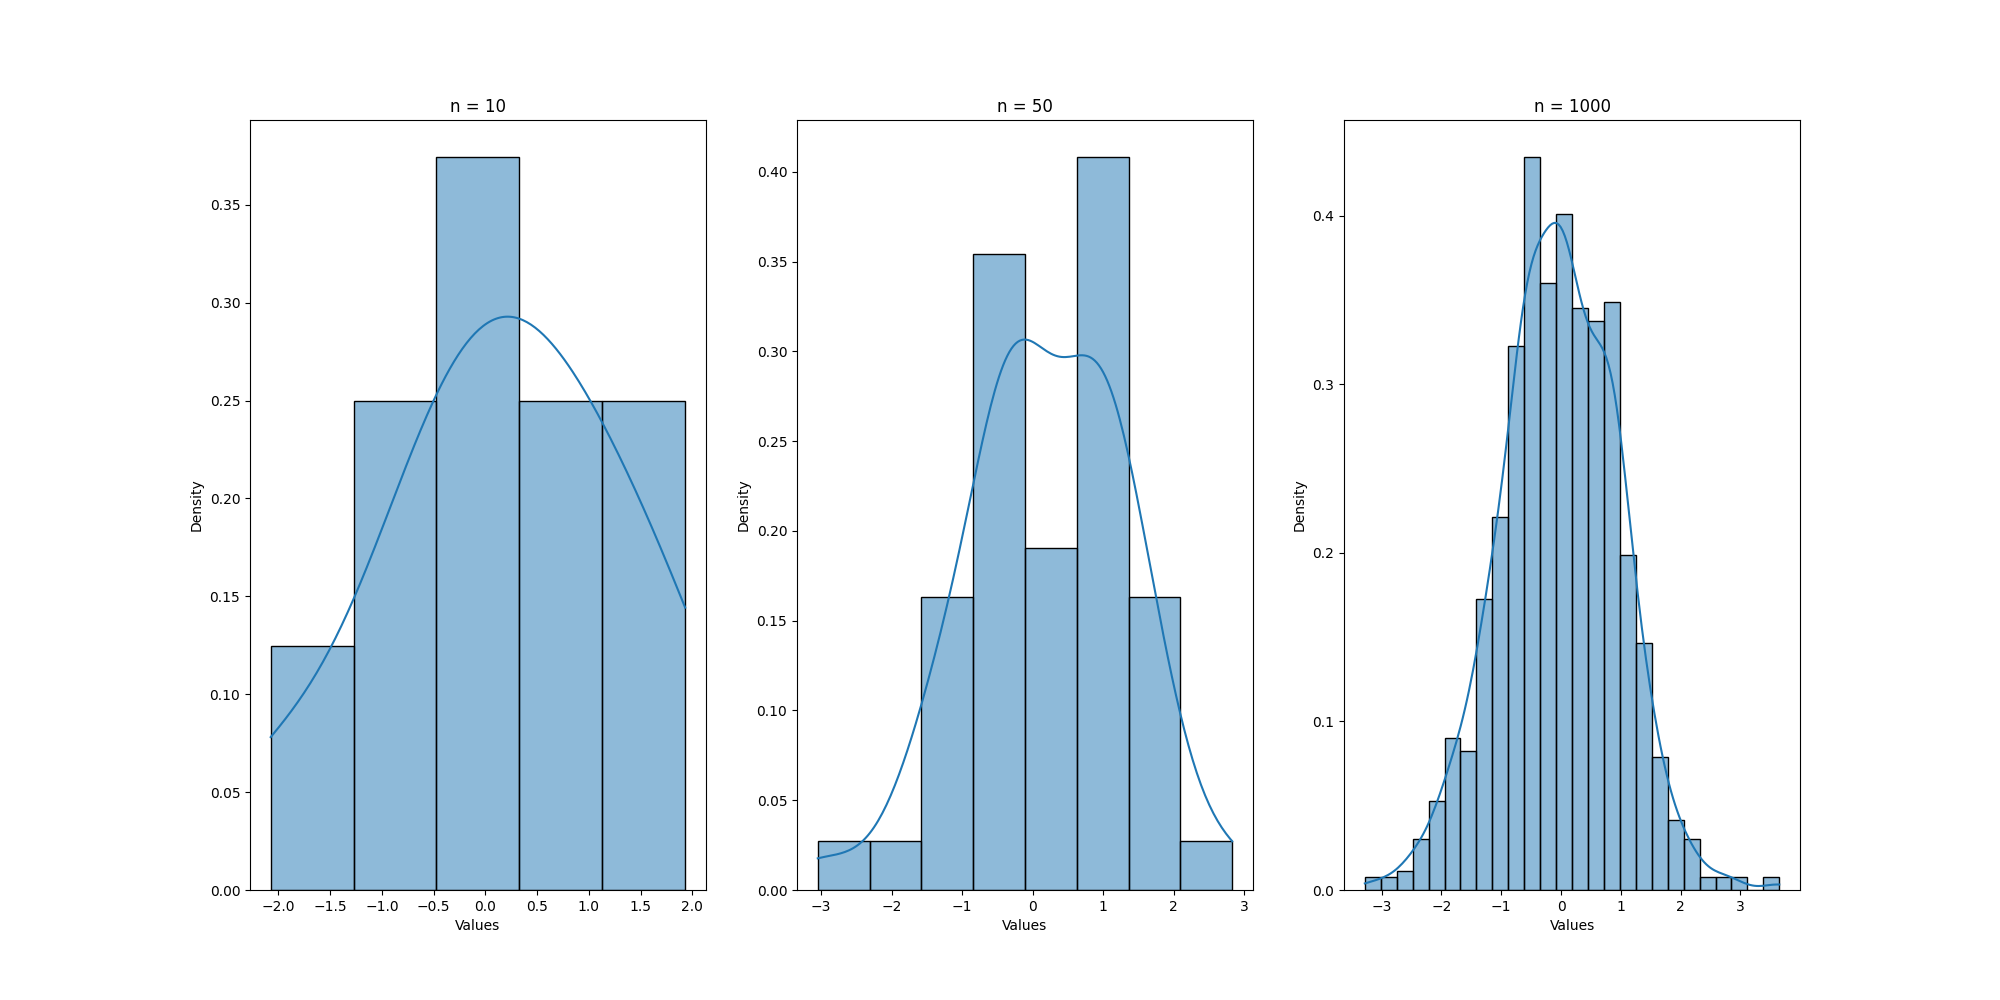
\includegraphics[width = 1.12\linewidth]{graphics/normal.png}
			\caption{Нормальное распределение \ \eqref{eq:normal}}
		\end{center}
	\end{figure}

	\begin{figure}[htbp!]
		\begin{center}
			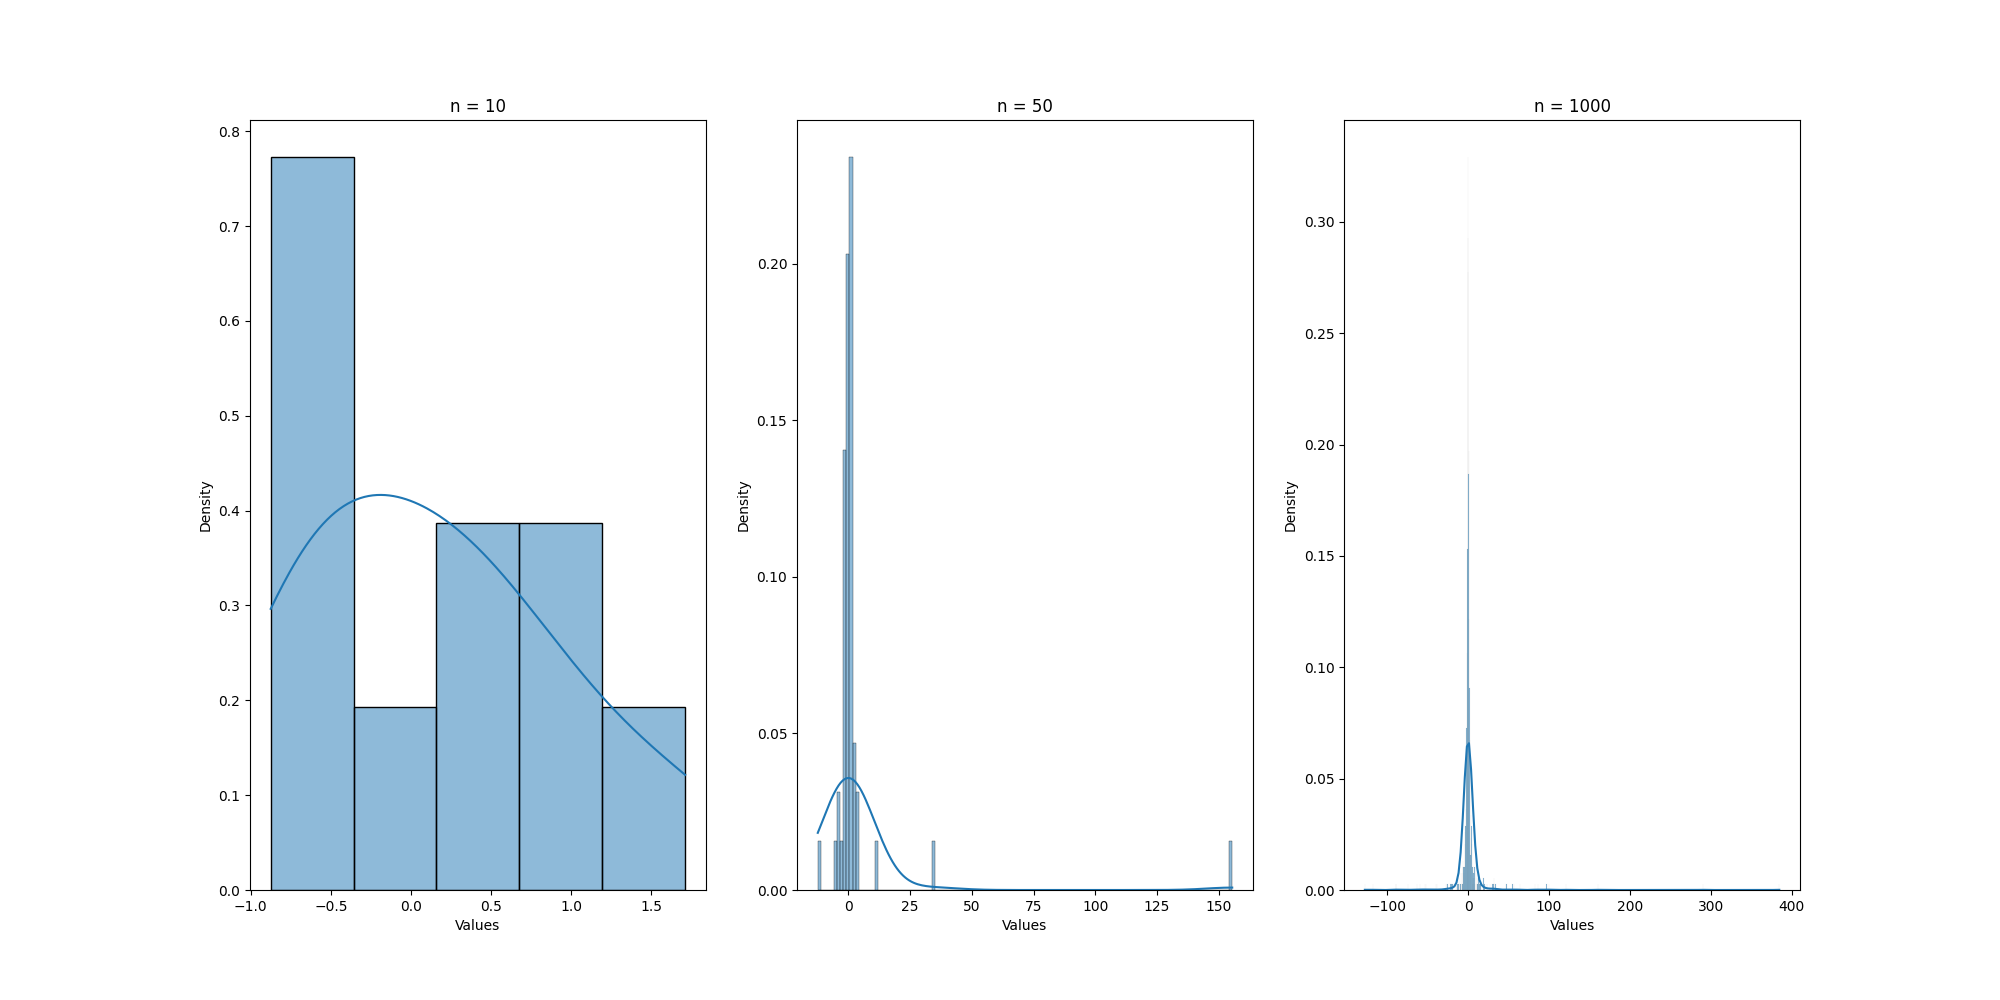
\includegraphics[width = 1.12\linewidth]{graphics/cauchy.png}
			\caption{Распределение Коши \ \eqref{eq:cauchy}}
		\end{center}
	\end{figure}

	\newpage

	\begin{figure}[htbp!]
		\begin{center}
			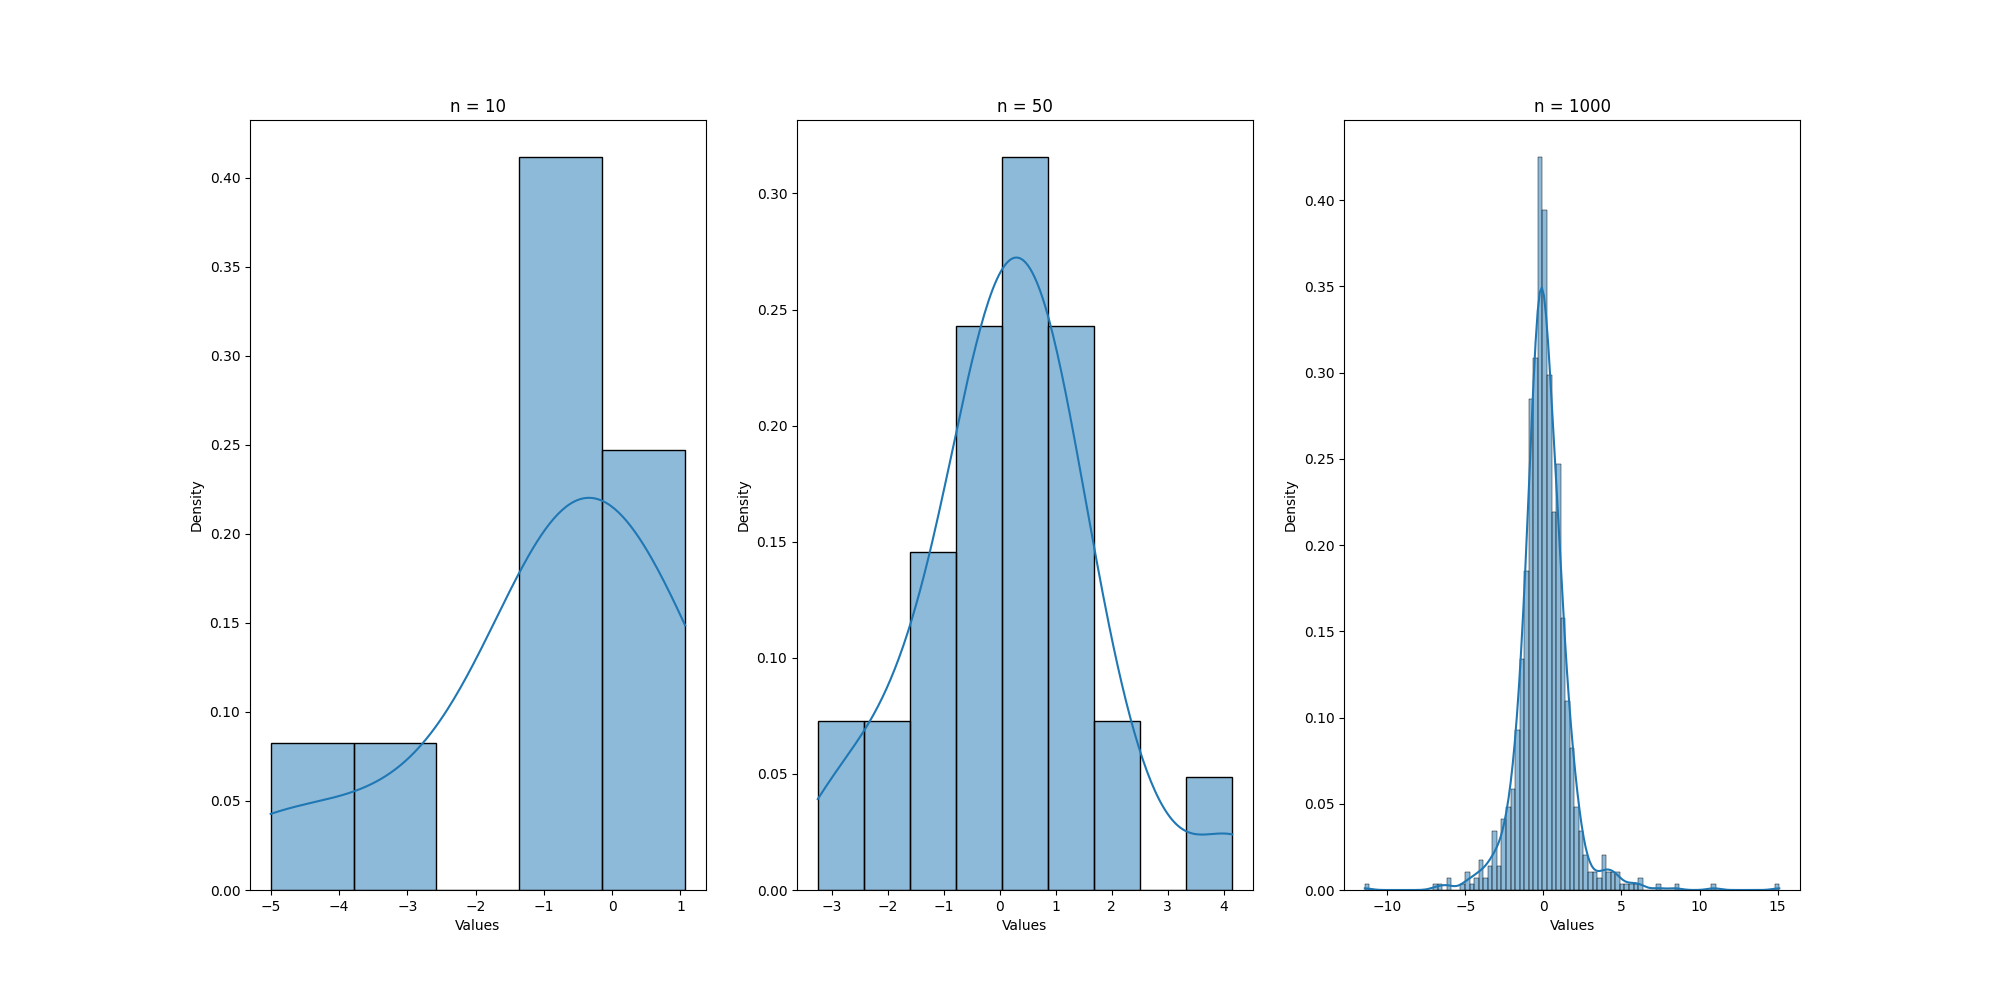
\includegraphics[width = 1.12\linewidth]{graphics/student.png}
			\caption{Распределение Стьюдента \ \eqref{eq:student}}
		\end{center}
	\end{figure}

	\begin{figure}[htbp!]
		\begin{center}
			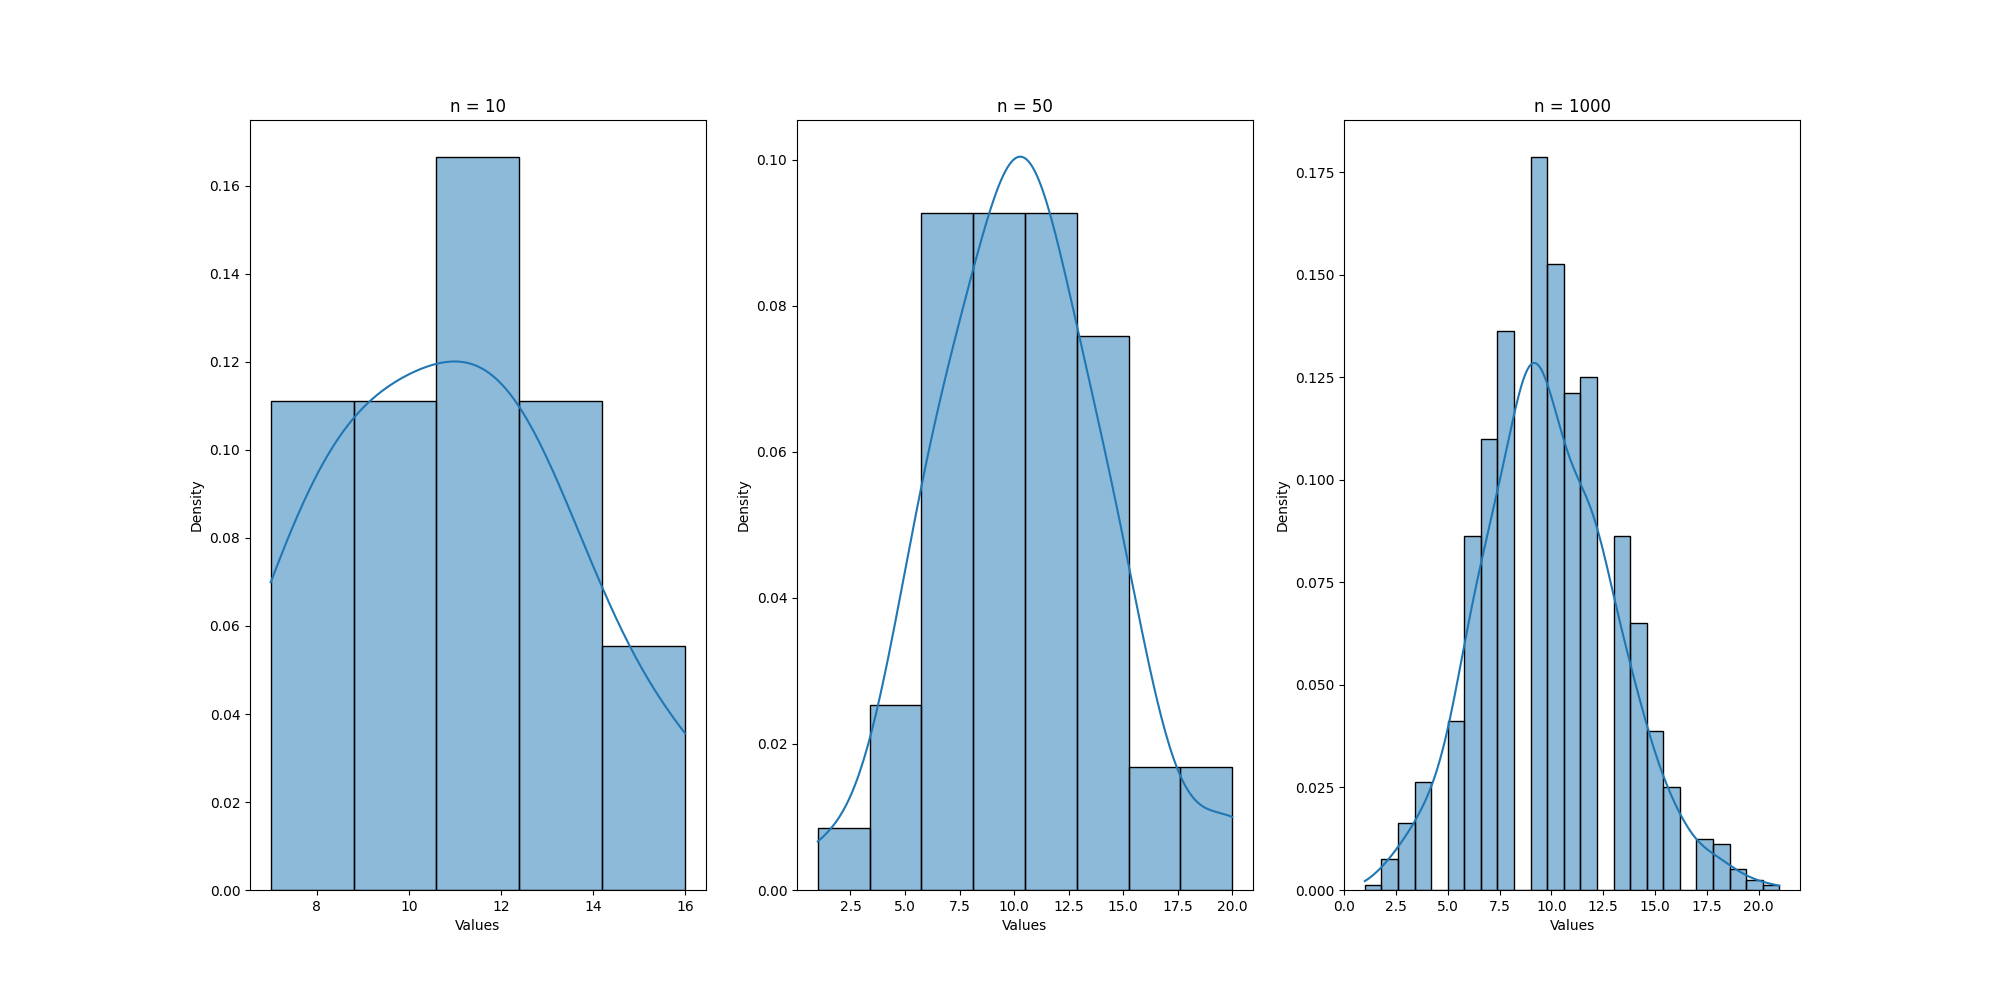
\includegraphics[width = 1.12\linewidth]{graphics/poisson.png}
			\caption{Распределение Пуассона \ \eqref{eq:poisson}}
		\end{center}
	\end{figure}

	\begin{figure}[htbp!]
		\begin{center}
			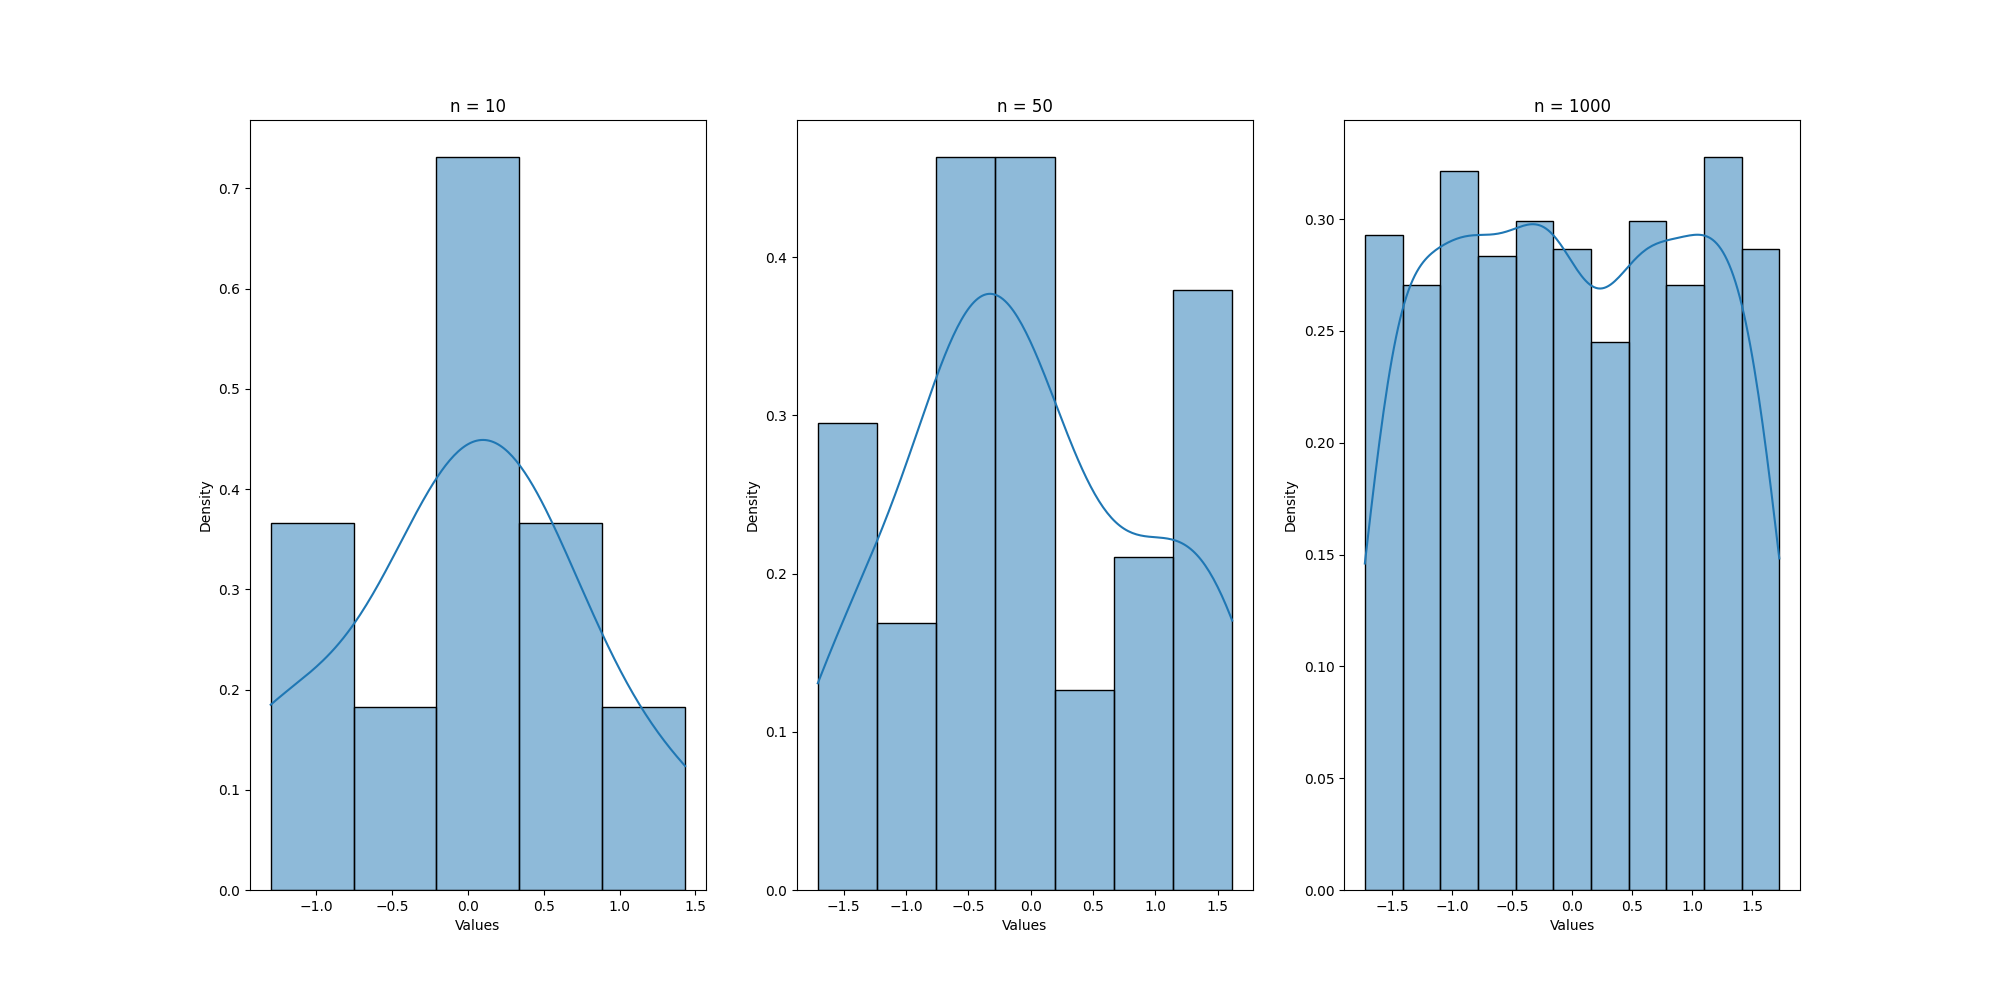
\includegraphics[width = 1.12\linewidth]{graphics/uniform.png}
			\caption{Равномерное распределение \ \eqref{eq:uniform}}
		\end{center}
	\end{figure}

	\newpage

	\subsection{Характеристики положения и рассеяния}

	\begin{table}[htbp!]
		\centering
		\begin{tabular}{ |c|c|c|c|c|c| }
			\hline
			n = 10 & & & & & \\
			\hline
			&$\overline{x}\ \eqref{eq:mean}$ & $med\ x \ \eqref{eq:median}$ & $z_{R} \ \eqref{eq:half_sum_of_extremal_elements}$ & $z_{Q} \ \eqref{eq:half_sum_of_quartiles}$ & $z_{tr} \ \eqref{eq:trimmed_mean}$\\
			\hline
			$E(z) \ \eqref{eq:expected_value}$ & -0.017466 & -0.019283 & -0.019494 & -0.014486 & -0.007937 \\
			\hline
			$D(z) \ \eqref{eq:dispersion} $ & 0.100879 & 0.142707 & 0.187775 & 0.115437 & 0.160836 \\
			\hline
			n = 50 & & & & & \\
			\hline
			&$\overline{x}\ \eqref{eq:mean}$ & $med\ x \ \eqref{eq:median}$ & $z_{R} \ \eqref{eq:half_sum_of_extremal_elements}$ & $z_{Q} \ \eqref{eq:half_sum_of_quartiles}$ & $z_{tr} \ \eqref{eq:trimmed_mean}$\\
			\hline
			$E(z) \ \eqref{eq:expected_value}$ & -0.007937 & 0.100879 & 0.142707 & 0.187775 & 0.115437 \\
			\hline
			$D(z) \ \eqref{eq:dispersion}$ & 0.009941 & 0.015535 & 0.095586 & 0.012392 & 0.020005 \\
			\hline
			n = 1000 & & & & & \\
			\hline
			&$\overline{x}\ \eqref{eq:mean}$ & $med\ x \ \eqref{eq:median}$ & $z_{R} \ \eqref{eq:half_sum_of_extremal_elements}$ & $z_{Q} \ \eqref{eq:half_sum_of_quartiles}$ & $z_{tr} \ \eqref{eq:trimmed_mean}$\\
			\hline
			$E(z) \ \eqref{eq:expected_value}$ & 0.000038 & -0.001779 & -0.002971 & 0.001002 & -0.000085 \\
			\hline
			$D(z) \ \eqref{eq:dispersion}$ & 0.000985 & 0.001682 & 0.061385 & 0.001243 & 0.001939 \\
			\hline
		\end{tabular}
		\caption{Нормальное распределение}
		\label{table:1}
	\end{table}

	\begin{table}[htbp!]
		\centering
		\begin{tabular}{ |c|c|c|c|c|c| }
			\hline
			n = 10 & & & & & \\
			\hline
			&$\overline{x}\ \eqref{eq:mean}$ & $med\ x \ \eqref{eq:median}$ & $z_{R} \ \eqref{eq:half_sum_of_extremal_elements}$ & $z_{Q} \ \eqref{eq:half_sum_of_quartiles}$ & $z_{tr} \ \eqref{eq:trimmed_mean}$\\
			\hline
			$E(z) \ \eqref{eq:expected_value}$ & -4.724165 & -0.015986 & -23.612109 & -0.015176 & -8.310631 \\
			\hline
			$D(z) \ \eqref{eq:dispersion} $ & 11477.749749 & 0.337081 & 286469.541418 & 1.163577 & 31698.450396 \\
			\hline
			n = 50 & & & & & \\
			\hline
			&$\overline{x}\ \eqref{eq:mean}$ & $med\ x \ \eqref{eq:median}$ & $z_{R} \ \eqref{eq:half_sum_of_extremal_elements}$ & $z_{Q} \ \eqref{eq:half_sum_of_quartiles}$ & $z_{tr} \ \eqref{eq:trimmed_mean}$\\
			\hline
			$E(z) \ \eqref{eq:expected_value}$ & 0.781733 & 0.012225 & 37.029997 & 0.008637 & 0.857304 \\
			\hline
			$D(z) \ \eqref{eq:dispersion}$ & 431.900044 & 0.025323 & 1060046.375320 & 0.055008 & 167.707860 \\
			\hline
			n = 1000 & & & & & \\
			\hline
			&$\overline{x}\ \eqref{eq:mean}$ & $med\ x \ \eqref{eq:median}$ & $z_{R} \ \eqref{eq:half_sum_of_extremal_elements}$ & $z_{Q} \ \eqref{eq:half_sum_of_quartiles}$ & $z_{tr} \ \eqref{eq:trimmed_mean}$\\
			\hline
			$E(z) \ \eqref{eq:expected_value}$ & -0.336134 & -0.001532 & -129.057477 & -0.001540 & -0.049715 \\
			\hline
			$D(z) \ \eqref{eq:dispersion}$ & 240.553988 & 0.002310 & 50362265.313181 & 0.004735 & 174.261104 \\
			\hline
		\end{tabular}
		\caption{Распределение Коши}
		\label{table:2}
	\end{table}

	\begin{table}[htbp!]
		\centering
		\begin{tabular}{ |c|c|c|c|c|c| }
			\hline
			n = 10 & & & & & \\
			\hline
			&$\overline{x}\ \eqref{eq:mean}$ & $med\ x \ \eqref{eq:median}$ & $z_{R} \ \eqref{eq:half_sum_of_extremal_elements}$ & $z_{Q} \ \eqref{eq:half_sum_of_quartiles}$ & $z_{tr} \ \eqref{eq:trimmed_mean}$\\
			\hline
			$E(z) \ \eqref{eq:expected_value}$ & 0.016265 & 0.004667 & 0.040925 & 0.014315 & 0.000750 \\
			\hline
			$D(z) \ \eqref{eq:dispersion} $ & 0.259126 & 0.183832 & 1.659319 & 0.184564 & 0.431912 \\
			\hline
			n = 50 & & & & & \\
			\hline
			&$\overline{x}\ \eqref{eq:mean}$ & $med\ x \ \eqref{eq:median}$ & $z_{R} \ \eqref{eq:half_sum_of_extremal_elements}$ & $z_{Q} \ \eqref{eq:half_sum_of_quartiles}$ & $z_{tr} \ \eqref{eq:trimmed_mean}$\\
			\hline
			$E(z) \ \eqref{eq:expected_value}$ & -0.002158 & -0.001389 & 0.021238 & 0.003592 & -0.016753 \\
			\hline
			$D(z) \ \eqref{eq:dispersion}$ & 0.026907 & 0.019051 & 9.893951 & 0.018478 & 0.052782 \\
			\hline
			n = 1000 & & & & & \\
			\hline
			&$\overline{x}\ \eqref{eq:mean}$ & $med\ x \ \eqref{eq:median}$ & $z_{R} \ \eqref{eq:half_sum_of_extremal_elements}$ & $z_{Q} \ \eqref{eq:half_sum_of_quartiles}$ & $z_{tr} \ \eqref{eq:trimmed_mean}$\\
			\hline
			$E(z) \ \eqref{eq:expected_value}$ & 0.000335 & -0.000238 & -0.054818 & 0.000162 & 0.000679 \\
			\hline
			$D(z) \ \eqref{eq:dispersion}$ & 0.002898 & 0.001903 & 32.527888 & 0.001944 & 0.005656 \\
			\hline
		\end{tabular}
		\caption{Распределение Стьюдента}
		\label{table:3}
	\end{table}

	\begin{table}[htbp!]
		\centering
		\begin{tabular}{ |c|c|c|c|c|c| }
			\hline
			n = 10 & & & & & \\
			\hline
			&$\overline{x}\ \eqref{eq:mean}$ & $med\ x \ \eqref{eq:median}$ & $z_{R} \ \eqref{eq:half_sum_of_extremal_elements}$ & $z_{Q} \ \eqref{eq:half_sum_of_quartiles}$ & $z_{tr} \ \eqref{eq:trimmed_mean}$\\
			\hline
			$E(z) \ \eqref{eq:expected_value}$ & 10.002500 & 9.874000 & 10.294500 & 9.917625 & 9.937000 \\
			\hline
			$D(z) \ \eqref{eq:dispersion} $ & 1.081944 & 1.477624 & 2.018020 & 1.283917 & 1.699309 \\
			\hline
			n = 50 & & & & & \\
			\hline
			&$\overline{x}\ \eqref{eq:mean}$ & $med\ x \ \eqref{eq:median}$ & $z_{R} \ \eqref{eq:half_sum_of_extremal_elements}$ & $z_{Q} \ \eqref{eq:half_sum_of_quartiles}$ & $z_{tr} \ \eqref{eq:trimmed_mean}$\\
			\hline
			$E(z) \ \eqref{eq:expected_value}$ & 10.013690 & 9.855500 & 10.896000 & 9.945125 & 10.013560 \\
			\hline
			$D(z) \ \eqref{eq:dispersion}$ & 0.095748 & 0.197370 & 0.957184 & 0.139817 & 0.204837 \\
			\hline
			n = 1000 & & & & & \\
			\hline
			&$\overline{x}\ \eqref{eq:mean}$ & $med\ x \ \eqref{eq:median}$ & $z_{R} \ \eqref{eq:half_sum_of_extremal_elements}$ & $z_{Q} \ \eqref{eq:half_sum_of_quartiles}$ & $z_{tr} \ \eqref{eq:trimmed_mean}$\\
			\hline
			$E(z) \ \eqref{eq:expected_value}$ & 10.005702 & 9.997000 & 11.627000 & 9.994000 & 10.004912 \\
			\hline
			$D(z) \ \eqref{eq:dispersion}$ & 0.010137 & 0.002991 & 0.634371 & 0.002964 & 0.020719 \\
			\hline
		\end{tabular}
		\caption{Распределение Пуассона}
		\label{table:4}
	\end{table}

	\begin{table}[htbp!]
		\centering
		\begin{tabular}{ |c|c|c|c|c|c| }
			\hline
			n = 10 & & & & & \\
			\hline
			&$\overline{x}\ \eqref{eq:mean}$ & $med\ x \ \eqref{eq:median}$ & $z_{R} \ \eqref{eq:half_sum_of_extremal_elements}$ & $z_{Q} \ \eqref{eq:half_sum_of_quartiles}$ & $z_{tr} \ \eqref{eq:trimmed_mean}$\\
			\hline
			$E(z) \ \eqref{eq:expected_value}$ & -0.005450 & -0.006939 & -0.005412 & -0.007901 & -0.015610 \\
			\hline
			$D(z) \ \eqref{eq:dispersion} $ & 0.104110 & 0.240206 & 0.044016 & 0.144291 & 0.172234 \\
			\hline
			n = 50 & & & & & \\
			\hline
			&$\overline{x}\ \eqref{eq:mean}$ & $med\ x \ \eqref{eq:median}$ & $z_{R} \ \eqref{eq:half_sum_of_extremal_elements}$ & $z_{Q} \ \eqref{eq:half_sum_of_quartiles}$ & $z_{tr} \ \eqref{eq:trimmed_mean}$\\
			\hline
			$E(z) \ \eqref{eq:expected_value}$ & -0.001915 & -0.006312 & -0.001349 & 0.001960 & -0.004766 \\
			\hline
			$D(z) \ \eqref{eq:dispersion}$ & 0.010019 & 0.029723 & 0.000599 & 0.014276 & 0.018935 \\
			\hline
			n = 1000 & & & & & \\
			\hline
			&$\overline{x}\ \eqref{eq:mean}$ & $med\ x \ \eqref{eq:median}$ & $z_{R} \ \eqref{eq:half_sum_of_extremal_elements}$ & $z_{Q} \ \eqref{eq:half_sum_of_quartiles}$ & $z_{tr} \ \eqref{eq:trimmed_mean}$\\
			\hline
			$E(z) \ \eqref{eq:expected_value}$ & 0.000470 & 0.000924 & -0.000133 & -0.000355 & -0.000387 \\
			\hline
			$D(z) \ \eqref{eq:dispersion}$ & 0.001014 & 0.003127 & 0.000005 & 0.001469 & 0.001887 \\
			\hline
		\end{tabular}
		\caption{Равномерное распределение}
		\label{table:5}
	\end{table}

	\newpage

	\section{Выводы}

	В процессе выполнения лабораторной работы был проведен анализ пяти уникальных распределений: нормальное, Коши, Стьюдента, Пуассона и равномерное.
	Были сгенерированы выборки разных объемов для каждого из них - 10, 50 и 1000 элементов.
	Были созданы гистограммы каждого распределения и нанесены на них графики плотности соответствующих распределений, что облегчило наглядное сопоставление формы распределения выборок с их теоретическими аналогами.
	Были также рассчитаны разные показатели положения и рассеяния для каждой выборки, включая выборочную среднюю величину, медиану, полусумму крайних элементов выборки, полусумму квартилей и усеченное среднее.
	Использовалась стандартная формула для оценки дисперсии. \\

	На основании полученных данных были сделаны следующие выводы:

	\begin{enumerate}
		\item В случае нормального распределения, оценки показателей положения и рассеяния становятся ближе к их теоретическим значениям по мере увеличения размера выборки.
		\item Для распределения Коши показатели положения и рассеяния менее стабильны и могут сильно отличаться от теоретических даже при больших размерах выборки.
		\item Распределение Стьюдента при небольших размерах выборки также демонстрирует определенную нестабильность оценок, однако с увеличением размера выборки результаты становятся более точными.
		\item Для распределения Пуассона и равномерного распределения, оценки показателей положения и рассеяния кажутся стабильными при любом объеме выборки.
		\item В общем, выборочное среднее является наиболее чувствительным к экстремальным значениям по сравнению с медианой, особенно в меньших выборках. Однако с увеличением размера выборки, влияние этих экстремальных значений на среднее значение уменьшается. В то же время, медиана обычно более устойчива к выбросам и мало варьирует с изменением размера выборки.
		\item Медиана является чувствительной к типу распределения: в нормальном и распределении Стьюдента медиана равна среднему, в распределении Коши она дает надежные, устойчивые к выбросам оценки, в Пуассоновском приближается к среднему, и в равномерном равна половине суммы минимального и максимального значений.
	\end{enumerate}
\end{document}
